%%%%%%%%%%%%%%%%%%%%%%%%%%%%%%  IEEEsample.tex
%%%%%%%%%%%%%%%%%%%%%%%%%%%%%%%%%%%%%%%%%
%%%%%%%%%%%%%%%%%%%%%%%    More information: see the header of IEEEtran.sty
%%%%%%%%%%%%%%%%%%%%%%%
%%%%%%%%%%%%%%%%%%%%%%%%%%%%%%%%%%%%%%%%%%%%%%%%%%%%%%%%%%%%%%%%%%%%%%%%%%%%%%%%
%%%%

\documentclass[11pt,twoside, onecolumn]{IEEEtran}
%\documentclass[conference]{IEEEtran}

%%%\IEEEoverridecommandlockouts

\usepackage[ruled]{./algorithm2e}
%%for algorithm2e package, label has to be following caption in the same line!!!
\renewcommand{\algorithmcfname}{ALGORITHM}
\SetAlFnt{\small}
\SetAlCapFnt{\small}
\SetAlCapNameFnt{\small}
\SetAlCapHSkip{0pt}
\IncMargin{-\parindent}



%% \RequirePackage{times}
%% \RequirePackage{algorithmic}
%% \PassOptionsToPackage{boxed}{algorithm}
%% \RequirePackage{algorithm}
%% \RequirePackage{multicol}
%\renewcommand{\algorithmicrequire}{\textbf{Inputs:}}
%\renewcommand{\algorithmicensure}{\textbf{Outputs:}}
%\DeclareMathAlphabet{\mathtsl}{OT1}{ptm}{m}{sl}

%\def\BibTeX{{\rm B\kern-.05em{\sc i\kern-.025em b}\kern-.08em1
%    T\kern-.1667em\lower.7ex\hbox{E}\kern-.125emX}}

%\newtheorem{theorem}{Theorem}
%\newtheorem{lemma}{Lemma}
%\newtheorem{example}{Example}
%\newtheorem{corollary}{Corollary}

\RequirePackage{amssymb, mathptm}
\usepackage{amsbsy}
\usepackage{graphicx}
\usepackage{helvet}
\usepackage{enumerate}
\usepackage{amsmath}
\usepackage{amsfonts}
\usepackage{graphicx}
\usepackage{multirow}
\usepackage{subfig}
\usepackage{comment}



%%indent in algorithm


%\setcounter{page}{1}


% New command for the table notes.
\def\tabnote#1{{\small{#1}}}

% New command for the line spacing.
\newcommand{\ls}[1]
    {\dimen0=\fontdimen6\the\font
     \lineskip=#1\dimen0
     \advance\lineskip.5\fontdimen5\the\font
     \advance\lineskip-\dimen0
     \lineskiplimit=.9\lineskip
     \baselineskip=\lineskip
     \advance\baselineskip\dimen0
     \normallineskip\lineskip
     \normallineskiplimit\lineskiplimit
     \normalbaselineskip\baselineskip
     \ignorespaces
    }
%\renewcommand{\algorithmicrequire}{\textbf{Input:}}
%\renewcommand{\algorithmicensure}{\textbf{Output:}}

\newcommand{\beq}{\begin{equation}}
\newcommand{\eeq}{\end{equation}}
\newcommand{\beqarr}{\begin{eqnarray}}
\newcommand{\eeqarr}{\end{eqnarray}}
%\newcommand{\ov}{\overline}
\newcommand{\ov}{\bar}
\newcommand{\xor}{\bigoplus}
\newcommand{\Fm}{{\mathbb{F}}}



%the following is for space before and after align or other equation environment.

%%
\newtheorem{Algorithm}{Algorithm}[section]
\newtheorem{Definition}{Definition}[section]
\newtheorem{Example}{Example}[section]
\newtheorem{Proposition}{Proposition}[section]
\newtheorem{Lemma}{Lemma}[section]
\newtheorem{Theorem}{Theorem}[section]
\newtheorem{Corollary}{Corollary}[section]
\newtheorem{Conjecture}{Conjecture}[section]
\newtheorem{Problem}{Problem}[section]
\newtheorem{Notation}{Notation}[section]
\newtheorem{Setup}{Problem Setup}[section]
%%%

%%set spacing between table columns
\setlength{\tabcolsep}{3pt}

\begin{document}

%\thispagestyle{empty}
%\pagestyle{empty}

\ls{1.1}

\title{\large{\textsc{Report  on Algorithmic Tight Bound Analysis of
      Tree Metrics Approximation}}}
\author{Xiaojun Sun\\
A Final Project Report\\
as a satisfaction of requirement by Advanced Algorithms\\
Fall Semester 2013
}

%%\author{\IEEEauthorblockN{Jinpeng Lv and Priyank Kalla}\thanks{This work is sponsored in part by a grant from NSF \#CCF-546859.}
%\IEEEauthorblockA{Department of  Electrical and Computer Eng.\\
% University of Utah, Salt Lake City, UT-84112 \vspace{-0.3in}
 %\{lv, kalla\}@eng.utah.edu
% }
%\and
%\IEEEauthorblockN{Florian Enescu} \thanks{\normalsize  978-3-9810801-8-6/DATE12/$\copyright 2012$ EDAA}
%\IEEEauthorblockA{Department of Mathematics and Statistics\\
% Georgia State University,  Atlanta, GA 30302-4038 \vspace{-0.3in}
% fenescu@mathstat.gsu.edu
%} 
%
 
\maketitle

%\markboth{MS Proposal by Tim Pruss}{}
\newcommand{\Fq}{{\mathbb{F}}_{q}}
\newcommand{\Fkk}{{\mathbb{F}}_{2^k}}
\newcommand{\Fkkx}[1][x]{\ensuremath{\mathbb{F}}_{2^k}[#1]\xspace}
\newcommand{\Grobner}{Gr\"{o}bner\xspace}
\newcommand{\B}{{\mathbb{B}}}
\newcommand{\Z}{{\mathbb{Z}}}
\newcommand{\F}{{\mathcal{F}}}
\newcommand{\G}{{\mathcal{G}}}
\newcommand{\R}{\mathbb{R}}
%%%

\newcommand{\debug}[1]{\textcolor{gray}{[ #1 ]}}


%\thispagestyle{empty}

%%%%%%%%%%%%%%%%%%%% Include your files here %%%%%%%%%%%%%%%%%%%%%
\begin{abstract}
This report is discussing the key techniques of J. Fakcharoenphol el.'s journal paper\cite{thispaper}.
First, we learn about the importance of adopting tree metric approximating algorithms. Then two key
techniques are found: the CKR like algorithm to decompose a graph, as well as a region-growing like
algorithm to derandomize the probabilistic approximation. Former algorithm guarantees the expected
distortion among a set of trees has an upper bound $O(logn)$, latter one tells the existence of a single
tree whose average distortion also satisfies upper bound $O(logn)$. At last this paper concludes that
the $O(logn)$ distortion is a tight bound, thus can improve the performance of all tree metric approximation
applications. 
\end{abstract}

\section{Problem Description}
\label{sec:desc}
The problem this paper addressing is as its title states: to find a tight bound for the algorithm 
which approximate arbitrary metrics with tree metrics.
\subsection{Importance of Tree Metrics Approximation Problem}
For a lot of problems in both algorithmic research and real life, there exists a metric representation.
One example is the Traveling Salesman Problem (TSP). This problem can be represented by a weighted graph, as long as specifying a metric. If we want to solve this
problem, we will need to run over all possible tours and find out the optimal, because this is currently
proved to be a NP-hard problem. However, since metric space satisfies triangle inequality (will be
discussed later in section \ref{sec:basic}), a Spanning Tree Heuristic\cite{h_tsp} can be adopted,
the minimum spanning tree is taken, and bunch of polynomial-time algorithms can be applied on this spanning
tree to provide a n approximation to TSP.

\begin{figure}[hbt]
	\begin{center}
	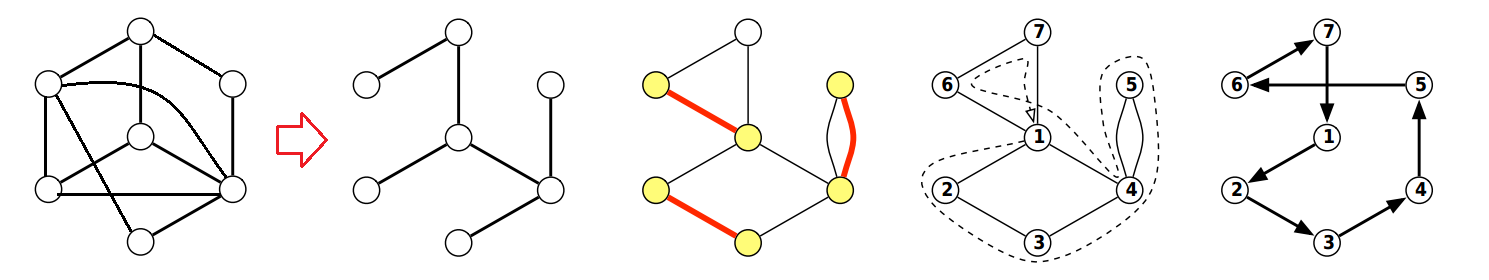
\includegraphics[scale=0.4]{h_tsp.png}
	\end{center}
	\caption{A spanning tree heuristic for TSP (revising from \cite{Jeff})}
	\label{fig:tsp}
\end{figure}

In nature, the spanning tree heuristic is a deterministic $\alpha$-approximation of a graph (without
loss of generality, we call it an arbitrary metric space) using tree metric.
This problem shows the importance of developing tree metrics approximation algorithms. Furthermore, if we could
embed an arbitrary metric into a tree with distortion $D$, then the optimal solution to this TSP
on the tree would be within $D$ of the optimal TSP tour on original input metric. As the distortion
be well-bounded at a lower level, the approximation algorithm will be further improved. More compelling
algorithmic applications of low distortion embeddings will be listed in section \ref{sec:potential}.

\subsection{History}
Approximations of metric spaces by "simpler" metric spaces has been intensively studied, both in
mathematics and computer science. 
"Embedding" is an important concept in these research areas,
it stands for a map from one metric space to another one, 
also can be defined in topology with geometry, algebra and domain theory with different sets/domains/fields. Johnson el.(1984)\cite{hilbert} discussed embeddings in Hilbert spaces at Functional
theory point of view; Graham el.(1985)\cite{zd} did some work about embeddings in $\Z^d$ in graph theory; moreover,
Linial el.(1994)\cite{realnorm} gave a research on low-distortion embeddings in low-dimensional real normed spaces.

As to research about tree metrics approximation, it origins from the paper by Cai el.(1995)\cite{Cai}
who gave out a tree spanner approximation to solve K-server problem. Soon, Bartal(1996)\cite{hst} introduced
an important structure called Hierarchically well Separated Tree (HST), and proved an arbitrary metric 
space can be $\alpha$-probabilistically-approximated with distortion $\alpha=O(log^2n)$, and lower bound is
$\Omega(logn)$(this will be extensively discussed in section \ref{sec:hst}). Later, Bartal(1998)\cite{bartal98}
developed Hierarchical Partition Metrics (HPM) based on HST fashion, and improved the bound of distortion
to $O(lognloglogn)$. 

Later, people began to focus on how to find a decomposition of graph which can 
benefit the tree metrics approximation. Calinescu el.(2001)\cite{CKR} gave an $O(logk)$ approximation
algorithm based on a linear programming relaxation for 0-extension problem (k is number of terminals), which is known as
CKR algorithm (will be introduced in section \ref{sec:CKR}). The partition algorithm of CKR
was improved by Fakcharoenphol el.(2003, actually authors of this paper)\cite{thispaper}, which is adopted finally
in this paper to provide a probabilistic graph decomposition algorithm which guarantees the expected distortion
have a upper bound $O(logn)$.

\subsection{Potential Applications}
\label{sec:potential}
Tree metrics approximation can help solve bunch of applications in a variety of fields. The following
problems already have reasonable approximation algorithm on trees, so if our goal (to approximate
arbitrary metrics with tree metrics) is attained, these problems can be easily solved for much broader
inputs.

{\bf The group Steiner tree} problem. Given a weighted graph and a collection of $k$ sets, find
a Steiner tree connecting at least one element from each set. Garg el.\cite{GKR98} give an $O(logklogn)$ approximation 
algorithm for trees.

{\bf Buy-at-bulk network design}. Given a weighted graph and a sub-linear function of cost
describing the edge cost as a function of the load on it. If given a sequence of pairs of nodes,
the objective is to find a path connecting each pair, and minimize the total load. Awerbuch el. \cite{AA97}
give an $O(1)$-approximation algorithm on trees.

{\bf The communication spanning tree} problem\cite{Hu74}. Given a metric space network with costs on edges, the
communication spanning tree problem is to find a spanning tree and minimize a weighted sum of tree distances
over all pairs of nodes. Graph decomposition fashion approach can be applied trivially to find
desired spanning tree.

Meantime, probabilistic approximation of metric spaces is of particular importance in the case of
on-line problems where randomization against oblivious adversaries is very powerful.

{\bf Metric task systems} consists of a set of states forming a metric space and a set of tasks 
associated with costs in the different states. The goal is to schedule state transitions in order to
minimize the total move and task costs. This problem has deterministic competitive ratio of $2n-1$, and
proved to have same upper and lower bound to the $(n-1)$-server problem on $n$ points.\cite{MMS88}

{\bf The K-server problem} consists of K-servers in a metric space, points are requested over time
and a server must be moved to the request location. The memoryless K-server algorithm for trees
developed by Chrobak\cite{CL91} is very efficient randomized algorithm comparing to traditional work function 
algorithm.

\section{Techniques from the Paper}
\subsection{Introduction to Basic Concepts}
\label{sec:basic}
There are some definitions to make, which is necessary to understand the argument of this paper.
\begin{Definition}
Given a set $X$ of points, a \emph{distance function} on $X$ is a map $d : X \times X \to \R_+$ that is symmetric,
and satisfies $d(i, i) = 0\ \forall i \in X$. The distance is said to be a $metric$ if the triangle inequality
holds, i.e.
$$d(i, j) \leq d(i, k) + d(k, j),
\ \forall\ i, j, k \in X.$$
\end{Definition}
Furthermore, a $metric\ space$ is a set
where metric for every element pair is defined. In graph theory, this “distance” is weight of a
path between arbitrary vertices. So any undirected weighted graph (UWG) could be interpreted
as a metric space. Given metric space $G = (V, d)$ as an UWG, $E$ is a set including all edges in $G$, $|
V| = n$, pick arbitrary vertices $u, v$ from V, denote the distance between them as $d(u, v)$, The property of metric space can also be written in 3 specifications:\par
(a) $d(u, v) \geq 0$, and $d(u, v) = 0$ if and only if $u = v$ ;\par
(b) $d(u, v) = d(v, u)$ (symmetry);\par
(c) $d(u, v) \leq d(u, w) + d(w, v)$ (triangle inequality).
\\
We also mentioned the "embedding" and "distortion" in section \ref{sec:desc}, they can be formalized as
following:
\begin{Definition}
Given metric spaces $(X, d)$ and $(X', d' )$, a map $f : X \to X'$ is called an \emph{embedding}.
\end{Definition}
\begin{Definition}
Given two metrics $(X, d)$ and $(X' , d' )$ and a map $f : X \to X'$ , the \emph{contraction} of $f$ is the
maximum factor by which distances are shrunk, i.e.,
$$\max_{x,y\in X}\frac{d(x,y)}{d'(f(x),f(y))}$$
the $expansion$ or $stretch$ of $f$ is the maximum factor by which distances are stretched:
$$\max_{x,y\in X}\frac{d'(f(x),f(y))}{d(x,y)}$$
and the $distortion$ of $f$ , denoted by $||f||_{dist}$ , is the product of the contraction and the expansion.
\end{Definition}
Easy to understand that "distortion" is the maximum difference between 2 metrics. 
 Next it is necessary to 
define the most important concept in the tree approximation algorithm: "$\alpha$-probabilistic approximation".
\begin{Definition}
A metric space $N$ over $V$, \emph{dominates} a metric space $M$ over $V$, if for
every $u,v\in V$, $d_N(u,v)\geq d_M(u,v)$.
\end{Definition}
\begin{Definition}
A metric space $N$ over $V$, $\alpha$-$approximates$ a metric space $M$ over $V$, if it dominates $M$
and for every $u,v\in V$, $d_N(u,v) \leq \alpha\cdot d_M(u,v)$.
\end{Definition}
\begin{Definition}
A set of metric spaces $\mathcal{S}$ over $V$, $\alpha$-$probabilistically$-$approximates$ a metric
space $M$ over $V$, if every metric space in $\mathcal{S}$ dominates $M$ and $\exists$ a probability 
distribution over metric space $N\in \mathcal{S}$ such that for every $u,v\in V$, 
$Ex(d_N(u,v))\leq \alpha\cdot d_M(u,v)$.
\end{Definition}
Here $Ex$ means expectations. Consider an optimization problem $\mathcal{P}$ defined on metric spaces,
the cost of solution for $\mathcal{P}$ can be expressed as a linear combination of distances between
vertices in metric space.\cite{bartal98} Use the linearity of expectations, if the probability distribution is known,
$\alpha$-probabilistic approximation is a good approximation when deterministic approximation is 
unavailable, just like the problem we concern: approximate an arbitrary metric with a single tree metric.

There is an example to explain how to calculate distortion $\alpha$, for an $\alpha$-probabilistic approximation for a tree to a graph.
\begin{Example}
\label{ex:ncycle}
Suppose we have a $n$-cycle graph, remove one edge randomly to get a tree. For each edge $(u,v)\in E$ on this 
tree, the probability of distant change is $\frac{1}{n}$, while probability for unchange is $\frac{n-1}{n}$.
So the expectation of distortion on one edge is (assume initial distance in n-cycle for neighbors are all 1,
the distortion is then equal to distance on tree metric space):
$$Ex(d_T(u,v)) = \frac{1}{n}\cdot (n-1) + \frac{n-1}{n} \cdot 1 = 2\frac{n-1}{n} \leq 2$$
We can assert that this n-cycle can be \emph{2-probabilistically-approximated} by a tree with uniform probability distribution.
\end{Example}
\subsection{Graph Decomposition and CKR Algorithm}
\label{sec:CKR}
Example \ref{ex:ncycle} is a good explanation on how to build a tree out of a graph by cutting some edges.
The graph decomposition techniques reply on a CKR-like procedure. The CKR algorithm is shown below:
\begin{algorithm}[hbt]
\SetAlgoNoLine
 \KwIn{A semi-metric space (where distinct vertices may have 0 distance) $G=(V,d)$, while every edge has corresponding distance greater than 1}
 \KwOut{A tree semi-metric space dominating original semi-metric space\\} %, a Gr\"{o}bner basis
  Choose a random permutation $\sigma$ of terminals(for 0-extension problem);\\
  Choose a real number $\alpha$ uniformly at random from $[1,2)$;\\
  \For{each vertex $v\in V$}
  {
  	$l \gets 1$\;
  	\While{$v$ has not yet been assigned a terminal} 
	{
		\If{$d(v,\sigma(l)) \leq \alpha R(v)$}
		{
			assign $v$ to terminal $\sigma(l)$;
		}
		$l\gets l + 1$;
	}
   }
\caption {The CKR Algorithm}\label{alg:CKR}
\end{algorithm}
In this algorithm $R(v)$ is the distance of {\it closest terminal of $v$} to {\it this terminal's closest terminal}. 
Terminal is a special set of vertices in multi-way cut problem which can be used as roots of tree.
More details such as 0-extension problem and semi-metric are reasoned in \cite{CKR}, they do not make any difference to the new algorithm. Here, the authors make some modifications to this CKR algorithm
to achieve graph decomposition. 

The procedure can be briefly described like below: use balls of different sizes to cut this graph, the first
ball's radius is $D_i$ which can contain all vertices. Then recursively choose vertices as centers to draw
balls in half of previous radius $D_{i-1} = \frac{D_i}{2}$. Once the circle (bound of ball) cuts any edges,
delete them, repeat drawing until every vertex is sitting within a ball, at this time 
we only keep edges from higher layer's center to lower layer's centers. Now doing same thing recursively
for each smaller ball with smaller radius $\frac{D_{i-1}}{2}$ (or in other words, go into lower layer $i-2$).
 Repeat this until every vertex is a center of a ball, all remaining edges and all vertices form a tree.
 
\begin{figure}[hbt]
	\begin{center}
	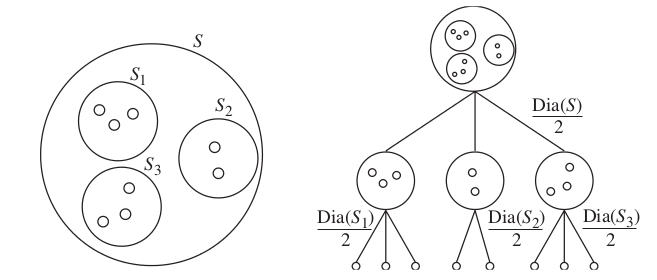
\includegraphics[scale=0.4]{laminar.png}
	\end{center}
	\caption{Brief procedure of graph decomposition by ball cutting\cite{thispaper}}
	\label{fig:laminar}
\end{figure}
We call this algorithm "FRT algorithm" in the same fashion of "CKR algorithm"(C,K,R are initials of authors).
We can see one main difference is the probability to choose ball radiuss, this will be important
in the tight bound analysis later in section \ref{sec:cutbound}.

\begin{algorithm}[hbt]
\SetAlgoNoLine
 \KwIn{A metric space $G=(V,d)$, while every edge has corresponding distance strictly greater than 1}
 \KwOut{A tree metric space dominating original metric space\\} %, a Gr\"{o}bner basis
  Choose a random permutation $\pi$ of all vertices;\\
  Choose a real number $\beta$ randomly from $[1,2]$ at distribution $p(x) = \frac{1}{xln2}$;\\
  $D_\delta \gets V$; $i\gets \delta-1$;\ \  /* $D$ means set of vertices in the ball, largest ball has radius $2^\delta$ */\\
  \While{$D_{i+1}$ has non-singleton clusters}
  {
  	$\beta_i \gets 2^{i-1}\beta$;\ \ /* Choose radius not exactly on powers of 2 */\\
  	\For{$l = 1,2,\dots,n$} 
	{
		\For{every cluster $S$ in $D_{i+1}$}
		{
			Create a new cluster consisting of all unassigned vertices in $S$ closer than $\beta_i$ to $\pi(l)$
		}

	}
	$i\gets i-1$;
   }
\caption {The FRT Algorithm}\label{alg:FRT}
\end{algorithm}
A graphical example of FRT decomposition is attached in APPENDIX section.
\subsection{k-Hierarchically well Separated Trees}
\label{sec:hst}
The definition of k-hierarchically well separated tree ($k$-HST) was first state in Bartal's paper\cite{hst}.
\begin{Definition}
A {\it k-hierarchically well separated tree} is defined as a rooted weighted tree with following properties:\par
(a) The edge weight from any node to each of its children is the same.\par
(b) The edge weights along any path from the root to a leaf are decreasing by a factor of at least $k$.
\end{Definition}
Obviously in FRT graph decomposition, the tree we construct is 2-HST, because: weights on tree edge in the
same layer are all $2^{i}$ (upper bound), and the radius shrinks by factor 2 when going down one layer.
Actually in \cite{bartal98}, 2-HST can be converted to any $k$-HST with distortion $O(k/logk)$, this
proves the FRT algorithm is able to be better utilized on more general applications 
even taking another factor rather than 2.

\section{Computational Analysis}
\subsection{Graph Decomposition Bound Analysis}
\label{sec:cutbound}
In section \ref{sec:CKR} we mentioned the brief procedure of graph partition method (FRT algorithm) used 
in this paper. In this section, we will prove that the expectation of tree metric distortion compared
to original graph has a $O(log n)$ bound.

The computation of expectation of distortion follows the method in example \ref{ex:ncycle}. As the proof
in this paper, we define to formalize:
\begin{Definition}
Center $w$ \emph{settles} the edge $(u,v)$ at level/layer $i$ if it is the first center to which at least one 
end of this edge ($u$ and $v$) get assigned.
\end{Definition}

From this definition, there is exactly one center settles any edge $(u,v)$ at any particular level.
Note that edge $(u,v)$ is in level $i$ means $u$ and $v$ first get separated to different clusters at level $i$.
Also a formal definition of "cut" can be made here:
\begin{Definition}
Center $w$ \emph{cuts} edge $(u,v)$ at level $i$ if it settles $(u,v)$ at this level, but exactly one
of $u,v$ is assigned to (included in ball) $w$ at level $i$.
\end{Definition}

One example of "cut" is in fig \ref{fig:cut}, $\pi(1)$ is the center of grey shaded ball, it has radius
$2^{i-1}\beta$. Assume this ball is the first ball we drew in this level, and there exists an edge
$(\pi(10),\pi(2))$. Since $\pi(10)$ is first time to be assigned to $\pi(1)$, we call $\pi(1)$ cuts
this edge at level $i-1$.

%%%%%%%%figure:cut here
\begin{figure}[hbt]
	\begin{center}
	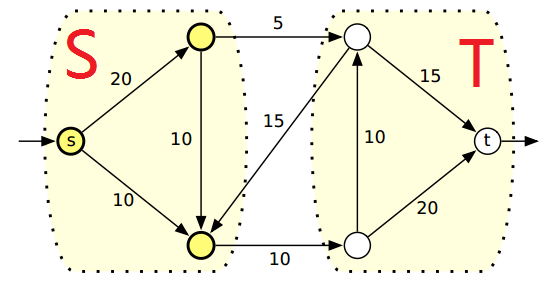
\includegraphics[scale=0.4]{cut.png}
	\end{center}
	\caption{Sample for hierarchically ball cutting (revised from \cite{thispaper})}
	\label{fig:cut}
\end{figure}

Then we can review the proof in this paper (part 2.3, p 490-492) step by step. First, it says 
\begin{Theorem}
If $w$ cuts
edge $(u,v)$, the tree length of this edge $(u,v)$ is about $2^{i+2}$.
\end{Theorem}

{\it Proof}\ \ 
Tree metric we need
always dominates original metric, so we need to estimate the maximum; current radius that cut $(u,v)$ is
$2^i$ maximum (please refer to FRT algorithm, $2^{i-1}\beta \leq 2^i$), so the distance between $u,v$ is
2 times of current diameter, i.e. $4\times 2^{i} = 2^{i+1}$. Fig \ref{fig:distance}(a) illustrates this
assert. 
In that figure, $u$ is assigned to center $w$, and there must exist a center $w'$ comes later (in the same
level or lower levels) to which $v$ is assigned. We know center $w$ cuts edge $(u,v)$ at level $i$,
then the radius of ball $w$ is $r$, the radius of ball $w'$ must satisfy $r'\leq r$. Note that
the distance between $w,w'$ should be less than $2r$, otherwise $(u,v)$ is located already in a higher level.
 So the largest possible distance of $u,v$ is $4r$.
$\Box$

Then the new distance counting on the tree metric space associated with center $w$ is denoted with $d_w^T(u,v)$.
Consider the center $w$ is arbitrarily taken from a set of vertices, it is necessary
to apply the upper bound on an arbitrary partition. Arrange a sequence of these centers $\{w_1, w_2, \dots, w_s,\dots, w_n\}$ in the order of $d_{w_1}^T(u,v) \leq d_{w_2}^T(u,v)\leq\cdots d_{w_s}^T(u,v)\leq \cdots d_{w_t}^T(u,v)$, $w_s$ is picked arbitrarily. Without loss of generality, assume $d(w_s,u)\leq d(w_s,v)$.
To satisfy $w_s$ cuts edge $(u,v)$, 2 conditions must be fulfilled:\\
(a) $d(w_s,u) \leq \beta_i < d(w_s,v)$ for some $i$;\\
(b) $w_s$ settles $(u,v)$ at level $i$.

The expectation of tree metric distance when condition (a) is fulfilled is:
\begin{align}
Ex\left(d_{w_s}^T(u,v)\ |\ d(w_s,u) \leq \beta_i < d(w_s,v)\right) &= \sum Pr(\beta_i\ lies\ in\ [\ d(w_s,u),d(w_s,v)\ ))\cdot d_{w_s}^T(u,v)\nonumber\\
&= \int_{d(w_s,u)}^{d(w_s,v)}\frac{1}{xln2}\cdot d_{w_s}^T(u,v)\cdot dx\nonumber
\end{align} 
note that the value of $d_{w_s}^T(u,v)$ has upper bound $2^{i+2} = 8\cdot 2^{i-1}\leq 8\cdot 2^{i-1}\beta = 8\beta_i$.

Condition (b) is fulfilled when $w_s$ is the first in sequence of $<w>$ which can settle $(u,v)$
at level $i$. Since $w_j$ defines a tree distance smaller than $w_s$ when $j<s$, with the same radius,
 $w_j$ can surely "settle" this edge at level $i$, an example is fig \ref{fig:distance}(b). In this
 example we assume tree distance is $d(w_s,u)+d(w_s,v)$, easy to observe that any center $w_j$
 configuring a shorter tree distance is sitting at a location satisfying the definition of
 "settle" edge $(u,v)$ when applying radius $\beta_i$.
 
 %figure distances
 \begin{figure}[hbt]
	\begin{center}
	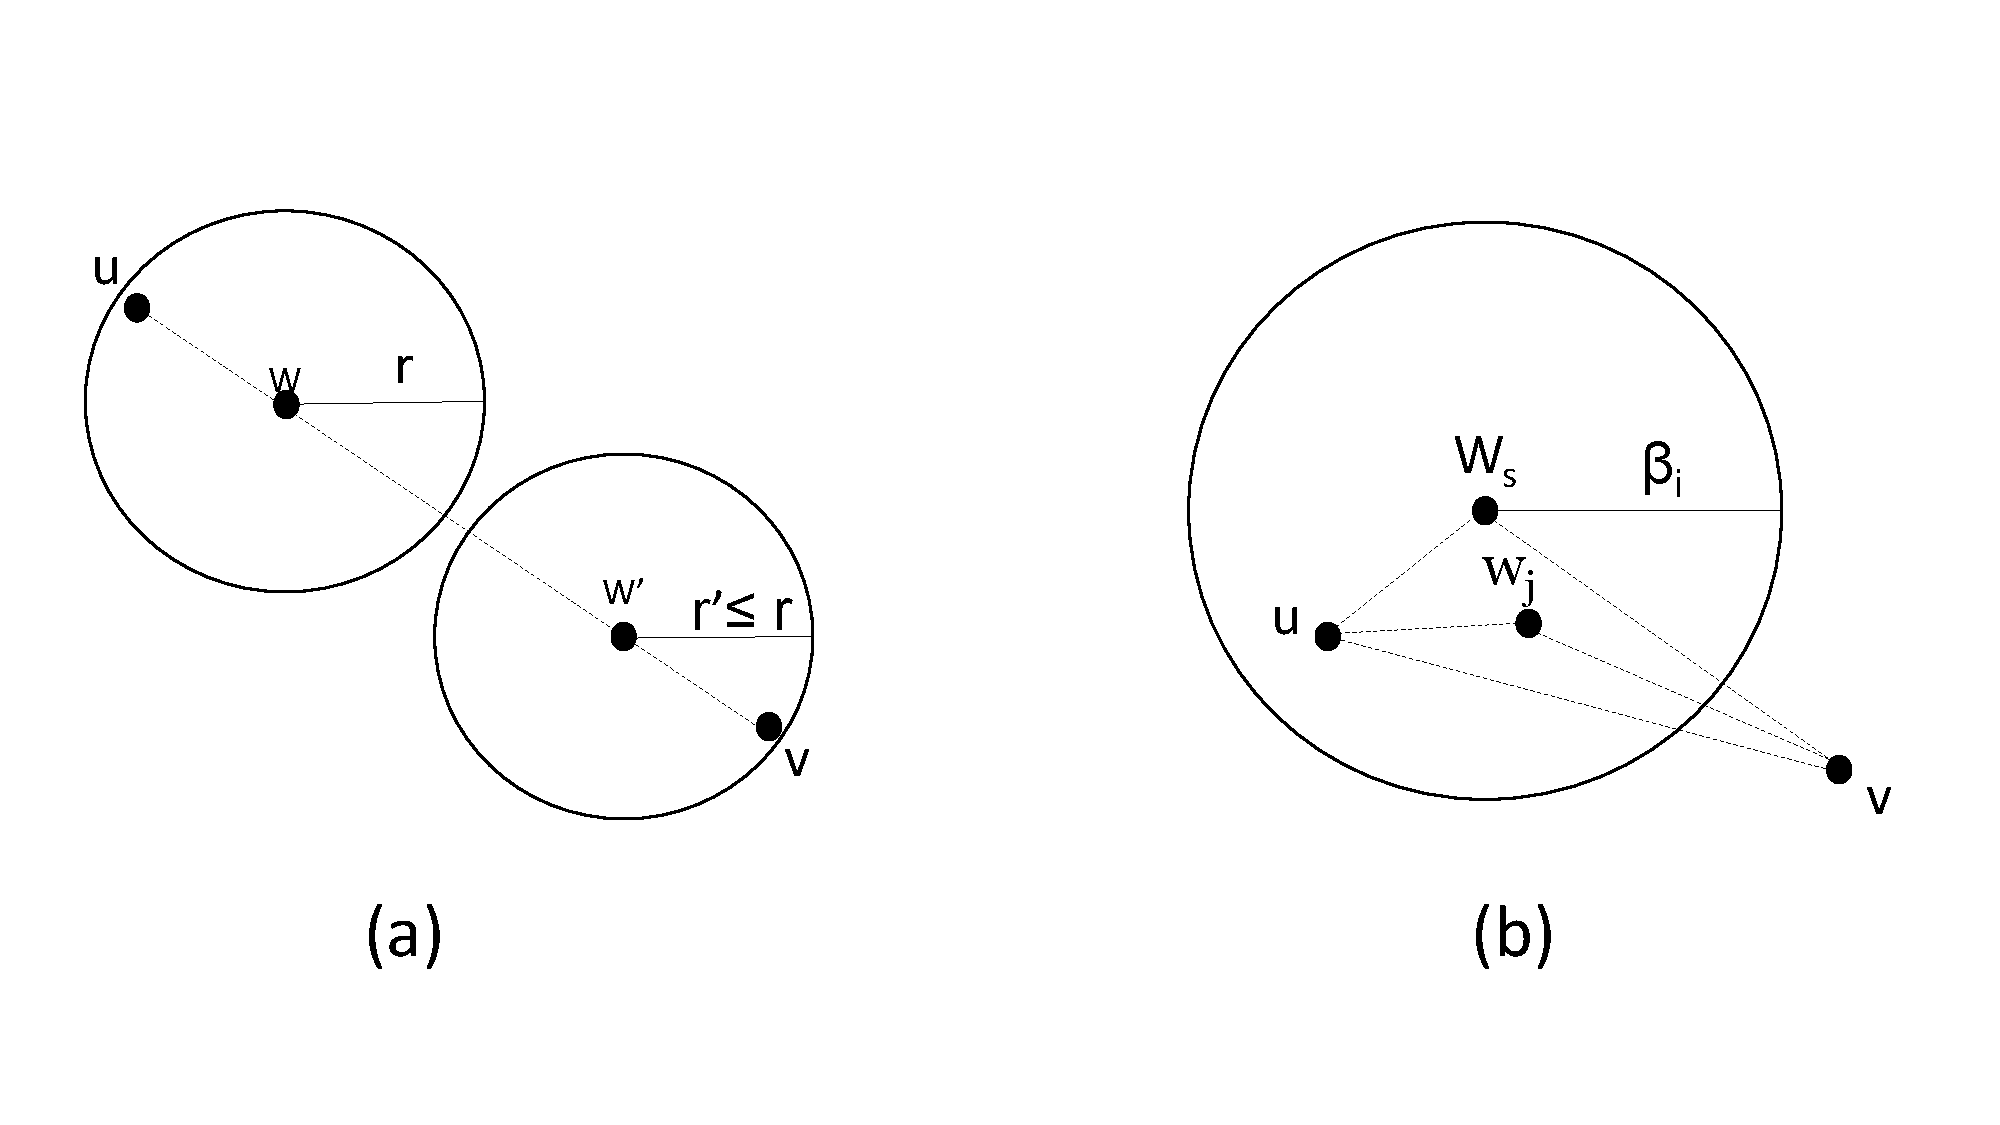
\includegraphics[scale=0.4]{fig_distance.pdf}
	\end{center}
	\caption{Examples for partition upper bound proof}
	\label{fig:distance}
\end{figure}
 
Concluding above arguments, in a consecutive sequence $\{w_1,w_2,\dots,w_s\}$ every element can
settle $(u,v)$ if it is the first center selected at level $i$ under condition (a). Considering
that $w_j$ may also settle $(u,v)$ even $j>s$ and $w_s$ is randomly chosen, probability
$$Pr\text{(condition\ (b) } | \text{ condition\ (a))} \leq \frac{1}{s}$$
this is a conditional probability. Following assertion $Pr(A\ and\ B) = Pr(A)\cdot Pr(B|A)$,
probability for center $w_s$ to cut (u,v) is 
$$\frac{1}{s}\int_{d(w_s,u)}^{d(w_s,v)}\frac{1}{xln2}\cdot d_{w_s}^T(u,v)\cdot dx$$
since $\frac{1}{s}$ is irrelevant with variable $x$, it can be directly multiplied into
expectation calculation, so the expected tree metric distance between $u,v$ through $w_s$ is
\begin{align}
Ex\left(d_{w_s}^T(u,v)\right)
&\leq \int_{d(w_s,u)}^{d(w_s,v)}\frac{1}{xln2}\cdot 8x\cdot\frac{1}{s} dx\nonumber\\
&=\frac{8}{sln2}(d(w_s,v)-d(w_s,u))\\
&\leq \frac{8d(u,v)}{sln2}\ \ \ \text{(triangle\ inequality)}
\end{align} 

$w_s$ is randomly chosen from sequence containing $n$ vertices. Using linearity of expectation,
the expected tree metric distance is bounded by
$$Ex(d_T(u,v)) \leq \sum_{s=1}^{n}\frac{8d(u,v)}{sln2} = O(logn)\cdot d(u,v)$$

The conclusion is
\begin{Theorem}
The distribution over tree metrics resulting from FRT algorithm $O(logn)$-probabilistically-approximates the original metric $d$.
\end{Theorem}
\subsection{Derandomization Bound Analysis}
Derandomization means that FRT algorithm not only provide a set of tree metrics with desired expectation
on distortion, but also could actually give a single tree metric such that its distortion is bounded by $O(logn)$.

To generalize, assume for each edge $(u,v)$ there is weight $c_{uv}$ assigned on it. 
We want to prove that
\begin{Proposition}
The FRT algorithm can find a tree metric space $d^T$ such that $(V,d^T)$ dominates original metric space
$G = (V,d)$
and satisfies $$\sum_{u,v\in V}c_{uv}\cdot d^T(u,v)\leq O(logn)\sum_{u,v\in V}c_{uv}\cdot d(u,v)$$
\end{Proposition}

In order to formalize, we can define
\begin{Definition}
Given an edge $e = (u,v)$ of length $d_e$ and weight $c_e$, the \emph{volume} of the edge is $d_e\cdot c_e$,
the \emph{sum\ of volume} $W = \sum_ec_ed_e$ corresponding to a set of qualified edges.
\end{Definition}

Using the definition of volume, it is easy to further define the following concepts vital in our proof.

\begin{Definition}
\emph{Ball} is a set of vertices located in a ball with center $t$ and radius $r$, denoted by $B(t,r)$.
The \emph{volume of neighborhood} $W(t,r)$ is computed by following criteria:\par
(a) edge $e=(u,v)$ with both ends in $B(t,r)$ contributes $c_ed_e$ to $W(t,r)$;\par
(b) edge $e=(u,v)$ with exactly one end such as $u$ in $B(t,r)$ contributes $c_e(r-d(t,u))$ to $W(t,r)$;\par
(c) edge $e=(u,v)$ with no ends in $B(t,r)$ contributes 0 to $W(t,r)$;\par
\emph{Cut volume} is denoted as $c(t,r)=\sum_{u\in B(t,r),v\notin B(t,r)}c_{uv}$ representing total weight of
edges cut by $B(t,r)$.
\end{Definition}

Based on above definitions, the proof in this paper can be reproduced. First, this assertion is proved:
\begin{Theorem}
There are radii $r_i: 2^{i-1}\leq r_i < 2^i$ such that $\sum_i\frac{c(t,r_i)}{W(t,r_i)}\cdot 2^i \leq O(logn)$
if $W$ is polynomial function of size $n$.
\end{Theorem}

The proof is very detailed in this paper already (part 3.1, p491), using region growing lemma from Garg el.\cite{Garg}
and contradiction. Then the author relaxed pre-condition that $W$ has to be polynomial function of 
size $n$ by find the actual upper bound of $W$. The largest edge length is $O(n)$, and unit volume
also affects the total volume linearly ($O(n)$), so the unit neighborhood volume on unit edge length $W_0 = W(t,1)$ is at least $(O(n\cdot n))^{-1} = \Omega(1/n^2)$ times total volume $W$, ratio $W/W_0$ is bounded
by $O(n^2)$, then $ln(n^2) = O(logn)$, the results with assumption still stand.

Above theorem is used to calculate the deterministic upper bound distortion of FRT algorithm.
Let $t$ be the center that maximizes $W(t,2^i)$ ($2^i$ is highest level maximum radius as mentioned in 
section \ref{sec:cutbound}). The FRT algorithm cut out $B(t,r_i)$ ($r_i$ is chosen in this level w.r.t. $t$),
and the new tree metric edge has length upper bound $2^{i+2}$ as discussed.

Recall the inequality in our proposition, $c_{uv}\cdot d^T(u,v) \leq c(t,r_i)\cdot 2^{i+2}$ for one edge at level $i$, 
$\sum_{u,v\in V}c_{uv}\cdot d(u,v) = W(t,r_i)$ according to definition. Sum up for all possible reached levels:
$$\frac{\sum_{u,v\in V}c_{uv}\cdot d^T(u,v)}{\sum_{u,v\in V}c_{uv}\cdot d(u,v)}=\sum_i\frac{c(t,r_i)}{W(t,r_i)}\cdot 2^{i+2} \leq 4ln\frac{W(t,2^{i+2})}{W(t,2^i)} \leq 8ln\frac{W}{W(t,1)} = O(log(n)),$$
our proposition is proved. Note here $t$ is chosen to guarantee it can still cut some edge with unit(minimum)
length 1 to form unit volume $W(t,1)$.

In conclusion:
\begin{Theorem}
FRT algorithm returns a 2-hierarchically well separated tree metric $d_T$ such that\par
(a) $\forall u,v \in V, d_T(u,v)\geq d(u,v)$;\par
(b) $\sum_{u,v\in V}c_{uv}\cdot d^T(u,v)\leq O(logn)\sum_{u,v\in V}c_{uv}\cdot d(u,v)$.
\end{Theorem}
\subsection{Computational Complexity Analysis}
In algorithm \ref{alg:FRT}, there are 3 cycles exploiting every vertices, the time complexity is 
$O(n^3)$, a polynomial time complexity.

\section{Further Developments on this Paper}
\subsection{Improvements on Relevant Applications}
\label{sec:app}
All applications we mentioned in \ref{sec:potential} and listed in Part 4 in this paper (we are discussing)
get an improvement on their performance since the upper bound of distortion is optimized. Moreover,
its graph decomposition approach also inspires some now approximations like spatial approximation in
metric labeling problem in image processing\cite{metriclabel} and trip planing about big data\cite{plan}.

In graph theory the low-stretch spanning tree is also discussed as an important topic\cite{lowspan}.
\subsection{Formalization and Refinement on Theory}
Some refinements are made on the FRT algorithm, especially on the probability distribution to select 
ball radii, such as Cai\cite{RMOP}. However, since the tight bound can be applied generally in
similar approximation algorithms, there is no improvement on further constraining the distortion.

And Shalekamp relaxed the distribution assumption made in this FRT algorithm, and directly gave a proof
for the tight bound, this is a big progress to formalize the tree approximation algorithms\cite{FRT}.

\section{My Comments}
The tree approximation algorithm is a good approach to solve some NP-hard problems in graph theory,
thus to find a tight bound of the tree metric distortion is important to optimize lots of approximation 
algorithms. The derandomization process guarantees its correctness for on-line problems. In conclusion,
this paper is innovative and vital enough and worth 400+ citations.
%%%%%%%%%%%%%%%%%%%% The bibliography %%%%%%%%%%%%%%%%%%%%%%%%%%%%
\bibliographystyle{ieee}
\bibliography{advalg}

\end{document}

%%%%%%%%%%%%%%%%%%%%%%%%%%%  End of IEEEsample.tex  %%%%%%%%%%%%%%%%%%%%%%%%%%%
